\section{State of the Art}

\subsection{Current Software Solutions}
\begin{frame}{Current Software Solutions}
    \begin{itemize}
        \item{Current software solutions}
        \begin{itemize}
            \item{Current supervisors and management}
            \item{IATA Airport Handling Manual}
        \end{itemize}
        \item{Static solution}
        \item{Teams vs individual workers}
    \end{itemize}
\end{frame}

\begin{frame}{Current Software Solutions}
        \begin{figure}[H]
            \centering
            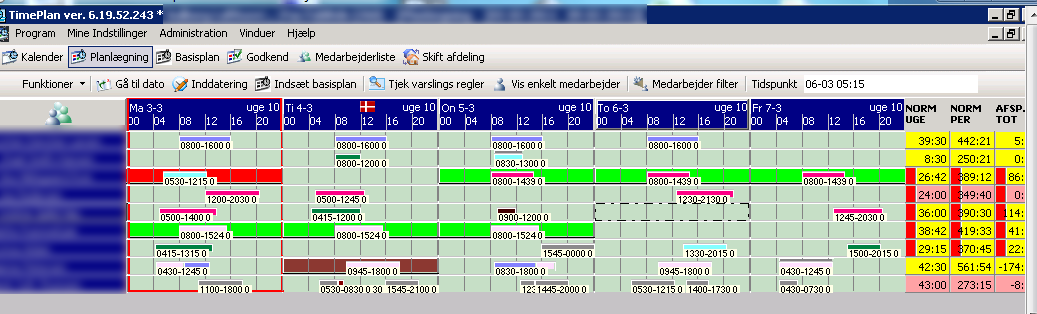
\includegraphics[width=230px]{Grafik/TimePlan}
            \caption{\footnotesize Software solution for time planning}
        \end{figure}
\end{frame}

\begin{frame}{Current Software Solutions}
        \begin{figure}[H]
            \centering
            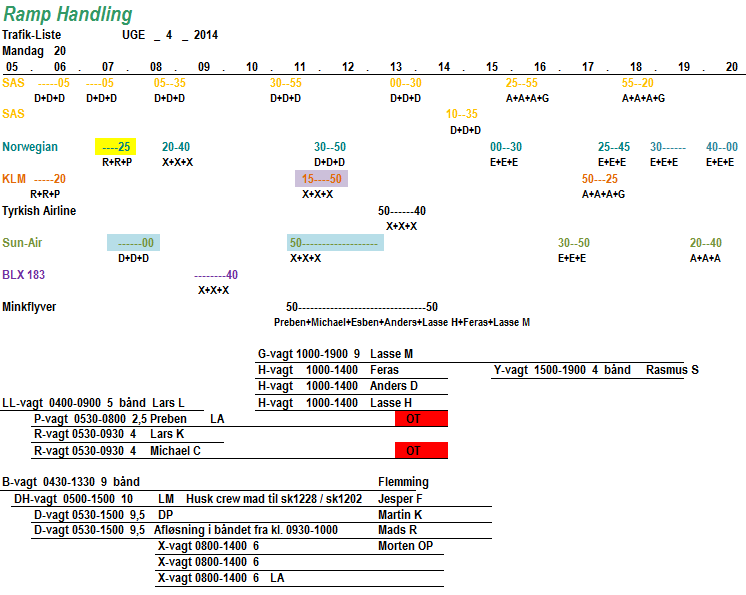
\includegraphics[width=230px]{Grafik/excelark}
            \caption{\footnotesize Excel page used by the ground handlers}
        \end{figure}
\end{frame}

\begin{frame}{Current Software Solutions}
    \begin{itemize}
        \item{Current software solutions}
        \begin{itemize}
            \item{Current supervisors and management}
            \item{IATA Airport Handling Manual}
        \end{itemize}
        \item{Static solution}
        \item{Teams vs individual workers}
    \end{itemize}
\end{frame}

\section{Summary}
\begin{frame}{Summary}
    \begin{itemize}
        \item{Summary}
        \item{Problem formulation}
    \end{itemize}

    \centerline{\tiny Human errors and accidents during a turnaround is a result of stressed, fatigued and}
    \centerline{\tiny unmotivated ground handlers, time pressure and bad communication, causing delays, damage to}
    \centerline{\tiny equipment and airplanes, personal injuries, loss of airtime and other unwanted, and expensive,}
    \centerline{\tiny annoyances for airlines and ground handling providers. How would it be possible to create a}
    \centerline{\tiny software solution that takes the different needs of the ground handlers into account, such as}
    \centerline{\tiny accounting for delays, by dynamically adapting their schedules to unplanned situations?}
\end{frame}

\section{Delimitation}
\begin{frame}{Delimitation}
    \begin{itemize}
        \item{Keyword: Dynamic solution}
        \item{Omitted factors}
        \item{Requirements}
    \end{itemize}

    \centerline{\tiny 1. The program should automatically generate, and update, the ground handlers' schedules.}
    \centerline{\tiny 2. The program has to take into account that some tasks cannot be performed simultaneously.}
    \centerline{\tiny 3. To minimize flight delays, the program has to be able to}
    \centerline{\tiny communicate the ground handlers' jobs to them, and directly notify them of changes.}
    \centerline{\tiny 4. The program has to be able to create teams dynamically.}
    \centerline{\tiny 5. The supervisors' should get the information about the}
    \centerline{\tiny performance reports automatically and courses of action should be recommended.}

\end{frame}